\documentclass{standalone}
\usepackage[dvipsnames]{xcolor}
\usepackage{tikz}
%\usepackage{pgfplots}
%\usepackage{pgfplotstable}
%\pgfplotsset{compat=1.5}
\usetikzlibrary{patterns}
\tikzstyle{v par}=              [dash pattern=on 10pt off 5pt,color=red!70,line width = 2pt]
\tikzstyle{z direction}=      [dash pattern=on 10pt off 5pt on 2pt off 5pt, color=Blue,line width = 2pt]

\begin{document}
{
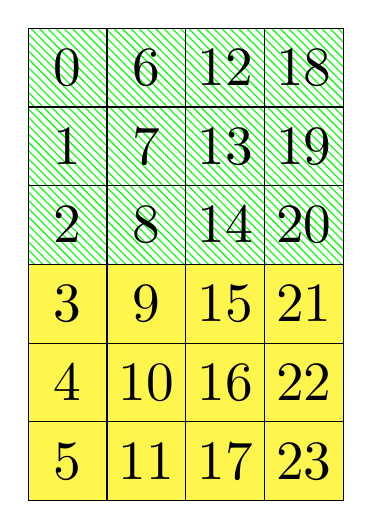
\begin{tikzpicture}
 
 \foreach \x in {0,...,2}
 {
  \foreach \y in {0,...,3}
  {
   \fill[yellow!70] (\y,\x) -- (\y,\x+1) -- (\y+1,\x+1) -- (\y+1,\x) -- (\y,\x);
   \draw (\y,\x) -- (\y,\x+1) -- (\y+1,\x+1) -- (\y+1,\x) -- (\y,\x);
   \pgfmathsetmacro\n{int((5-\x)+6*\y)}
   \node[scale=2] at (\y+0.5,\x+0.5) {\n};
  }
 }
 \foreach \x in {3,...,5}
 {
  \foreach \y in {0,...,3}
  {
   \draw[pattern=north west lines, pattern color=green] (\y,\x) rectangle (\y+1,\x+1);
   \draw (\y,\x) -- (\y,\x+1) -- (\y+1,\x+1) -- (\y+1,\x) -- (\y,\x);
   \pgfmathsetmacro\n{int((5-\x)+6*\y)}
   \node[scale=2] at (\y+0.5,\x+0.5) {\n};
  }
 }
\end{tikzpicture}
}
\end{document}
